% !Mode:: "TeX:UTF-8"
%% 请使用 XeLaTeX 编译本文.
% \documentclass{WHUBachelor}% 选项 forprint: 交付打印时添加, 避免彩色链接字迹打印偏淡. 即使用下一行:
 \documentclass[forprint]{shmtu}
\usepackage{listings}
\usepackage{xcolor}
\usepackage{graphicx}
\lstset{
	language=python,  %代码语言使用的是matlab
	frame=shadowbox, %把代码用带有阴影的框圈起来
	rulesepcolor=\color{red!20!green!20!blue!20},%代码块边框为淡青色
	keywordstyle=\color{blue!90}\bfseries, %代码关键字的颜色为蓝色,粗体
	commentstyle=\color{red!10!green!70}\textit,    % 设置代码注释的颜色
	showstringspaces=false,%不显示代码字符串中间的空格标记
	numbers=left, % 显示行号
	numberstyle=\tiny,    % 行号字体
	stringstyle=\ttfamily, % 代码字符串的特殊格式
	breaklines=true, %对过长的代码自动换行
	extendedchars=false,  %解决代码跨页时,章节标题,页眉等汉字不显示的问题
	%   escapebegin=\begin{CJK*},escapeend=\end{CJK*},      % 代码中出现中文必须加上,否则报错
	texcl=true}

\begin{document}
%%%%%%% 下面的内容, 据实填空.

\miji{ }                                      % 密级. 没有就空着.
\StudentNumber{202010311229} % 填写自己的学号

\title{面向对象课程设计\\图书管理系统}
\Etitle{面向对象课程设计\\图书管理系统} % 英文题目
\author{孙思进}                            % 作者名字
\Eauthor{Sijin Sun}            %作者英文名
\Csupervisor{金世双}        %指导教师中文名、职称
\Esupervisor{Teacher Kun Bi}     %指导教师英文名、职称
\Cmajor{计算机科学与技术}                  % 专业中文名
\Emajor{Computer Science and Technology}% 专业英文名
\Cschoolname{信息工程学院}          % 学院名
\Eschoolname{College of Information Engineering} %学院英文名. 不确定的话, 请看一下自己学院的网页上是怎么写的. 别搞错了!
\date{二〇二一年十一月}                    % 日期, 要注意和英文日期一致!!
\Edate{October, 2021}                       % 英文封面日期

%-----------------------------------------------------------------------------
\pdfbookmark[0]{封面}{title}         % 封面页加到 pdf 书签
\maketitle
\frontmatter
\pagenumbering{Roman}              % 正文之前的页码用大写罗马字母编号.
%-----------------------------------------------------------------------------
% !Mode:: "TeX:UTF-8"
\thispagestyle{empty}
\renewcommand{\baselinestretch}{1.5}  %下文的行距

\begin{cnabstract}
利用VC6.0开发工具开发一个图书管理系统系统。系统实现的功能模块有:用户登录、用户注册、数据库读取、数据库查询、借书、还书、查询书和升级权限的功能。
该系统的特色是轻量型和易开发,同时又有高可移植性的特点。系统操作实现的功能比较完善,人机界面实现简单,达到操作过程中的直观、方便、实用、安全等要求。系统具有一定的实用性。
实现了图书管理信息系统的图书检索、借阅管理、统计报表管理、图书个性化推荐等功能,能够有效提升图书馆的智能化信息管理和个性化信息服务水平。
\end{cnabstract}
\par
\vspace*{2em}

\cnkeywords{图书管理系统; 推荐系统; 信息管理}


%%====英文摘要==========================%


\begin{enabstract}
Using VC6.0 development tool to develop a library management system. The functional modules implemented by the system include: user login, user registration, database reading, database query, borrowing, returning, querying and upgrading permissions.

The system is characterized by light weight, easy development and high portability. The functions of the system operation are relatively perfect, and the realization of man-machine interface is simple, so as to meet the requirements of intuition, convenience, practicality and safety in the operation process. The system has certain practicability.

It realizes the functions of book retrieval, borrowing management, statistical report management and Book personalized recommendation of the library management information system, and can effectively improve the intelligent information management and personalized information service level of the library.
\end{enabstract}
\par
\vspace*{2em}
\enkeywords{Book Manage System;Recommend System;Information Management}
%%%%%-- Key words --------------------------------------%%%%%%%
%%%%-- 注意: 每个关键词之间用“;”分开,最后一个关键词不打标点符号    % 加入摘要, 申明.
%==========================把目录加入到书签==============================%%%%%%
\pdfbookmark[0]{目录}{toc}
\tableofcontents
\mainmatter %% 以下是正文
%%%%%%%%%%%%%%%%%%%%%%%%%%%--------main matter-------%%%%%%%%%%%%%%%%%%%%%%%%%%%%%%%%%%%%

\chapter{系统概述}
\section{系统设计背景}
随着时代的发展,知识改变了世界,人们越来越重视阅读,图书馆的人流量激增,图书馆的规模也随之扩大,馆藏书籍也逐渐增加,图书相关的信量的成倍增加,庞大的信息量使得传统的人工图书管理出现了诸多问题。

图书馆作为一种信息资源的集散地,图书和用户借阅资料繁多,包含很多的信息数据的管理,现今,有很多的图书馆都是初步开始使用,甚至尚未使用计算机进行信息管理。

根据调查得知,他们以前对信息管理的主要方式是基于文本、表格等纸介质的手工处理,对于图书借阅情况(如借书天数、超过限定借书时间的天数)的统计和核实等往往采用对借书卡的人工检查进行,对借阅者的借阅权限、以及借阅天数等用人工计算、手抄进行。

数据信息处理工作量大,容易出错;由于数据繁多,容易丢失,且不易查找。总的来说,缺乏系统,规范的信息管理手段。有必要建立一个图书管理系统,使图书管理工作规范化,系统化,程序化,避免图书管理的随意性,提高信息处理的速度和准确性,能够及时、准确、有效的查询和修改图书情况。
\\
\begin{itemize}
	\item 效率低。\\图书馆的藏书种类繁多,书籍数量也众多,若实用人工的方法将藏书准确地分门别类、快速检索效率是非常低的,往往到最后是终于查询到准确的图书信息馆中图书已经被他人借走。这个问题也会随着藏书的增加而越来越突出。
	\item 人工任务繁重且容易出错。\\大量的借还书任务,使得人工工作量大,随着图书馆越来越收到民众的欢迎,借书和还书的登记会超出预期,导致超负荷工作出现诸多问题。而且人工操作难免会有瑕疵出现。
	\item 图书管理不易。\\图书馆的藏书是会随着时代的推进而更新的,由于藏书的数量和种类的变化,加上自然损耗和人为破坏这些都需要图书管理来统计,如此庞大的工作人工是很难做到良好的效果的。
\end{itemize}

\section{系统设计目标}

本系统设计一个高效、便捷、实用的图书管理系统,将海量的图书信息用计算机科学技术进行系统地整理编排储存显得尤为重要。系统开发的总的设计目标是实现将图书管理变的系统化、自动化、规范化,对各种书籍和资料进行集中统一管理。主要用户涉及读者(借阅、归还、检索书籍、逾期缴费)和管理者(读者管理,书籍管理)。

\section{系统设计环境}

\subsection{主机}

测试系统和应用系统都安装了Windows 10 普通版,版本为1709。

\subsection{软件}

软件环境均列出在表\ref{tab:1}中。

\begin{table}[!htbp]
	\centering
	\caption{软件环境}
	\begin{tabular}{cccc}
		\hline
		序号 & 软件            & 版本     & 备注   \\ \hline
		1  & Visual Studio & 2019   & 编译环境 \\
		2  & Qt            & 4.10.0 & UI界面 \\ \hline
	\end{tabular}
	\label{tab:1}
\end{table}

\subsection{C++}
C++是C语言的继承,它既可以进行C语言的过程化程序设计,又可以进行以抽象数据类型为特点的基于对象的程序设计,还可以进行以继承和多态为特点的面向对象的程序设计。C++擅长面向对象程序设计的同时,还可以进行基于过程的程序设计,因而C++就适应的问题规模而论,大小由之。
C++不仅拥有计算机高效运行的实用性特征,同时还致力于提高大规模程序的编程质量与程序设计语言的问题描述能

\subsection{面向对象}
面向对象(Object Oriented)是软件开发方法,一种编程范式。面向对象的概念和应用已超越了程序设计和软件开发,扩展到如数据库系统、交互式界面、应用结构、应用平台、分布式系统、网络管理结构、CAD技术、人工智能等领域。面向对象是一种对现实世界理解和抽象的方法,是计算机编程技术发展到一定阶段后的产物。
面向对象是相对于面向过程来讲的,面向对象方法,把相关的数据和方法组织为一个整体来看待,从更高的层次来进行系统建模,更贴近事物的自然运行模式。

\subsection{QT}
Qt 是一个1991年由QtCompany开发的跨平台C++图形用户界面应用程序开发框架。它既可以开发GUI程序,也可用于开发非GUI程序,比如控制台工具和服务器。Qt是面向对象的框架,使用特殊的代码生成扩展(称为元对象编译器(Meta Object Compiler, moc))以及一些宏,Qt很容易扩展,并且允许真正地组件编程。
2008年,Qt Company科技被诺基亚公司收购,Qt也因此成为诺基亚旗下的编程语言工具。2012年,Qt被Digia收购。
2014年4月,跨平台集成开发环境Qt Creator 3.1.0正式发布,实现了对于iOS的完全支持,新增WinRT、Beautifier等插件,废弃了无Python接口的GDB调试支持,集成了基于Clang的C/C++代码模块,并对Android支持做出了调整,至此实现了全面支持iOS、Android、WP,它提供给应用程序开发者建立艺术级的图形用户界面所需的所有功能。基本上,Qt 同 X Window 上的 Motif,Openwin,GTK 等图形界面库和 Windows 平台上的 MFC,OWL,VCL,ATL 是同类型的东西。

\chapter{需求分析}

\section{系统需求分析}

为了进一步的学习面向对象课程的知识,把理论运用到实际的设计中,我们将具体完成以下任务。

\begin{itemize}
	\item 结合实际情况写出需求分析。
	\item 根据需求分析设计满足需求的界面。
	\item 为界面和控件设计具体的功能实现函数。
	\item 运行调试程序,对程序的缺陷进行修改。
	\item 调试无误,运行并测试具体的功能是否能满足实际需求。
\end{itemize}

结合实际情况,主要设计目标有:

\begin{itemize}
	\item 添加账户
	\item 修改账户
	\item 删除账户
	\item 查询书本(包括借还功能)
	\item 升级权限
\end{itemize}

\section{数据流图}

我们通过图\ref{pic:1}的结构表达了对数据流处理过程:

\begin{figure}[!htbp]
	\centering
	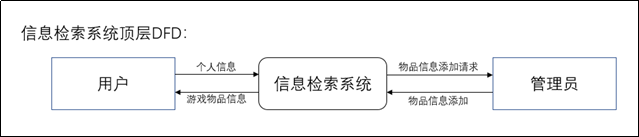
\includegraphics[height=0.1\textheight]{pic1.png}
	\caption{信息检索DFD}
	\label{pic:1}
\end{figure}

\section{数据字典}

\subsection{数据项}

数据项中我们使用了Acocount类作为父类,以此派生出User、Guest、Admin三个子类,他们拥有不同的权限。

同样,书本类使用Book作为主类,以此派生出Story、Education、Philosophy等不同书本类型的分类。

\begin{table}[!htbp]
	\caption{继承和派生关系}
	\begin{tabular}{llll}
		\hline
		bookname                        & author         & label & classname        \\ \hline
		Mom's Family Wall Calendar 2016 & Sandra Boynton & 3     & Calendars        \\
		(Harry Potter, Book 1)          & J.K. Rowling   & 4     & Children's Books \\
		Cracking the Coding Interview             & Gayle Laakmann McDowell & 6  & Computers \& Technology       \\
		The Wright Brothers                       & David McCullough        & 10 & Engineering \& Transportation \\
		Turn Your Weight Loss& Phil McGraw             & 11 & Health, Fitness \& Dieting    \\ \hline
	\end{tabular}
\end{table}

\subsection{数据字典}

本软件主要是用栈来存储数据,并再此的基础上进行查改删。

对于时间复杂度来说,栈的查找数量级在$O(n)$、修改的复杂度仅为$O(1)$。

\subsection{数据存储}

对于一个账号类,他的数据类型拥有账号、密码、权限;书本类中拥有书名、种类,标签、作者。

图书管理系统其本质就是对图书信息的管理,所以首先我们就必须弄清楚到底有那些信息,其次我们应该如何对这些信息进行系统地分类。结合实际情况进行合理分析,我们得出如下数据需求:

\begin{itemize}
	\item 借阅者\\借阅者编号,借阅者电话。
	\item 书籍\\书籍编号,书名,作者,出版日期,在库数,所在书库,入库日期,出库日期。
	\item 管理者\\管理者编号,负责书库。
	\item 借阅表\\借阅者编号,书籍编号,借出日期,到期日期,拖欠日期,罚款金额
	\item 销书清单\\书籍编号、管理者编号、书名、销书日期、销书数量
\end{itemize}

\section{概念结构设计}

通过将现代信息技术应用到图书馆管理工作中,我们能够充分发挥图书馆馆藏资源的价值,让所有数据能够被系统化地呈现在读者面前,以供读者进行分析和借阅。

另外,图片信息扫描系统让我们能够将一些珍贵的纸质图书转化为电子版图书,并且上传到计算机网络阅读平台,以供读者随时随地的通过网络平台进行阅读,让学习过程更加方便,不必受到时间和空间的约束。

与此同时,网络平台能够实现读者与读者之间的交流,共享阅读体会,这对于构建积极向上的阅读氛围有重要帮助。

\begin{figure}[!htbp]
	\centering
	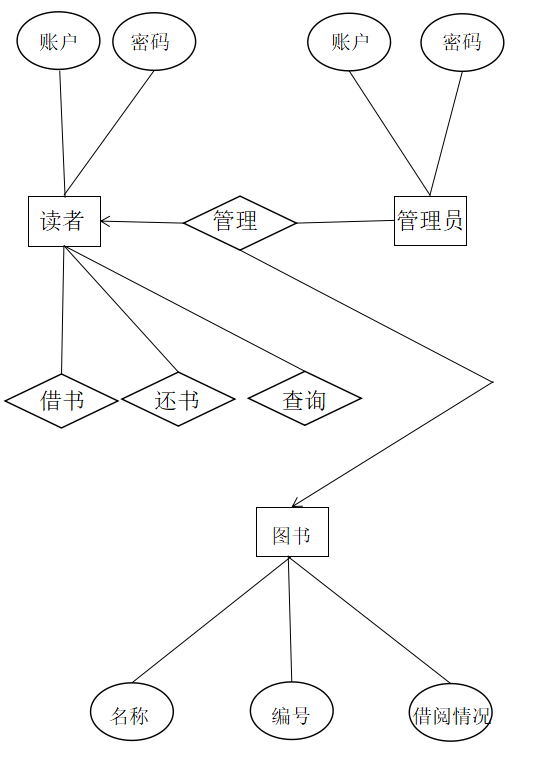
\includegraphics[height=0.3\textheight]{pic22.png}
	\caption{系统E-R图}
	\label{pic:22}
\end{figure}

为了更好地将现代信息技术融入图书馆管理工作之中,我们就必须要图书管理任务量化,做到有的放矢,围绕提升服务质量和服务效率来开展工作,立足于人民群众的实际阅读需求开展图书馆建设。计算机管理系统的应用够提升工作的透明度和规范度,并且减少了工作岗位人员的使用数量,极大地减少了人为失误状况的发生,让各项工作环节变得更加程序化,环环相扣,从而有效改变了传统图书管理中存在的不足。

所以,基于计算机的现代图书管理系统能够更好地收集用户信息,图书管理工作不仅仅是简单的借阅归还,而是朝着互联网方向和平台维护与升级的方向发展,这要求相关的计算机图书管理工作者不断优化平台建设,实现电子图书管理、网上平台借阅、用户行为习惯分析的内容,从而让整个服务更加多元化,促进图书馆的现代化建设。

通过上述分析,实现如上的功能,我们将系统流程图写在了图\ref{pic:2}。 
\begin{figure}[!htbp]
	\centering
	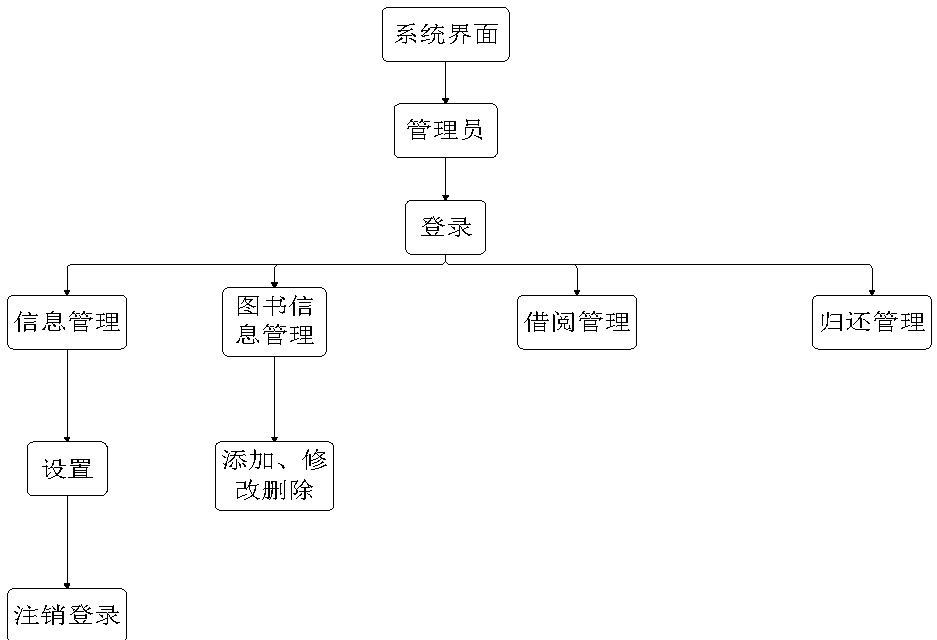
\includegraphics[height=0.2\textheight]{pic2.jpg}
	\caption{系统结构}
	\label{pic:2}
\end{figure}



\chapter{总体设计}

\section{数据库}

由于轻量化的使用,我们将数据格式保存为csv,通过csv的表格式读取,可以增加可读性,而csv文件后续也可以转化为数据库,为以后的升级创造了环境。

\section{系统功能设计}
高校图书馆在情报分析、资源组织揭示、知识服务等方面具备专业性优势,承担着高校智库的角色。高校图书馆在情报分析、资源组织揭示、知识服务等方面具备专业性优势,承担着高校智库的角色。高校图书馆在情报分析、资源组织揭示、知识服务等方面具备专业性优势,承担着高校智库的角色。

通过图\ref{pic:3}的架构图,我们设想一种除了图书管理系统以外的多媒体图书馆,为学生提供更多的功能。

\begin{figure}[!htbp]
	\centering
	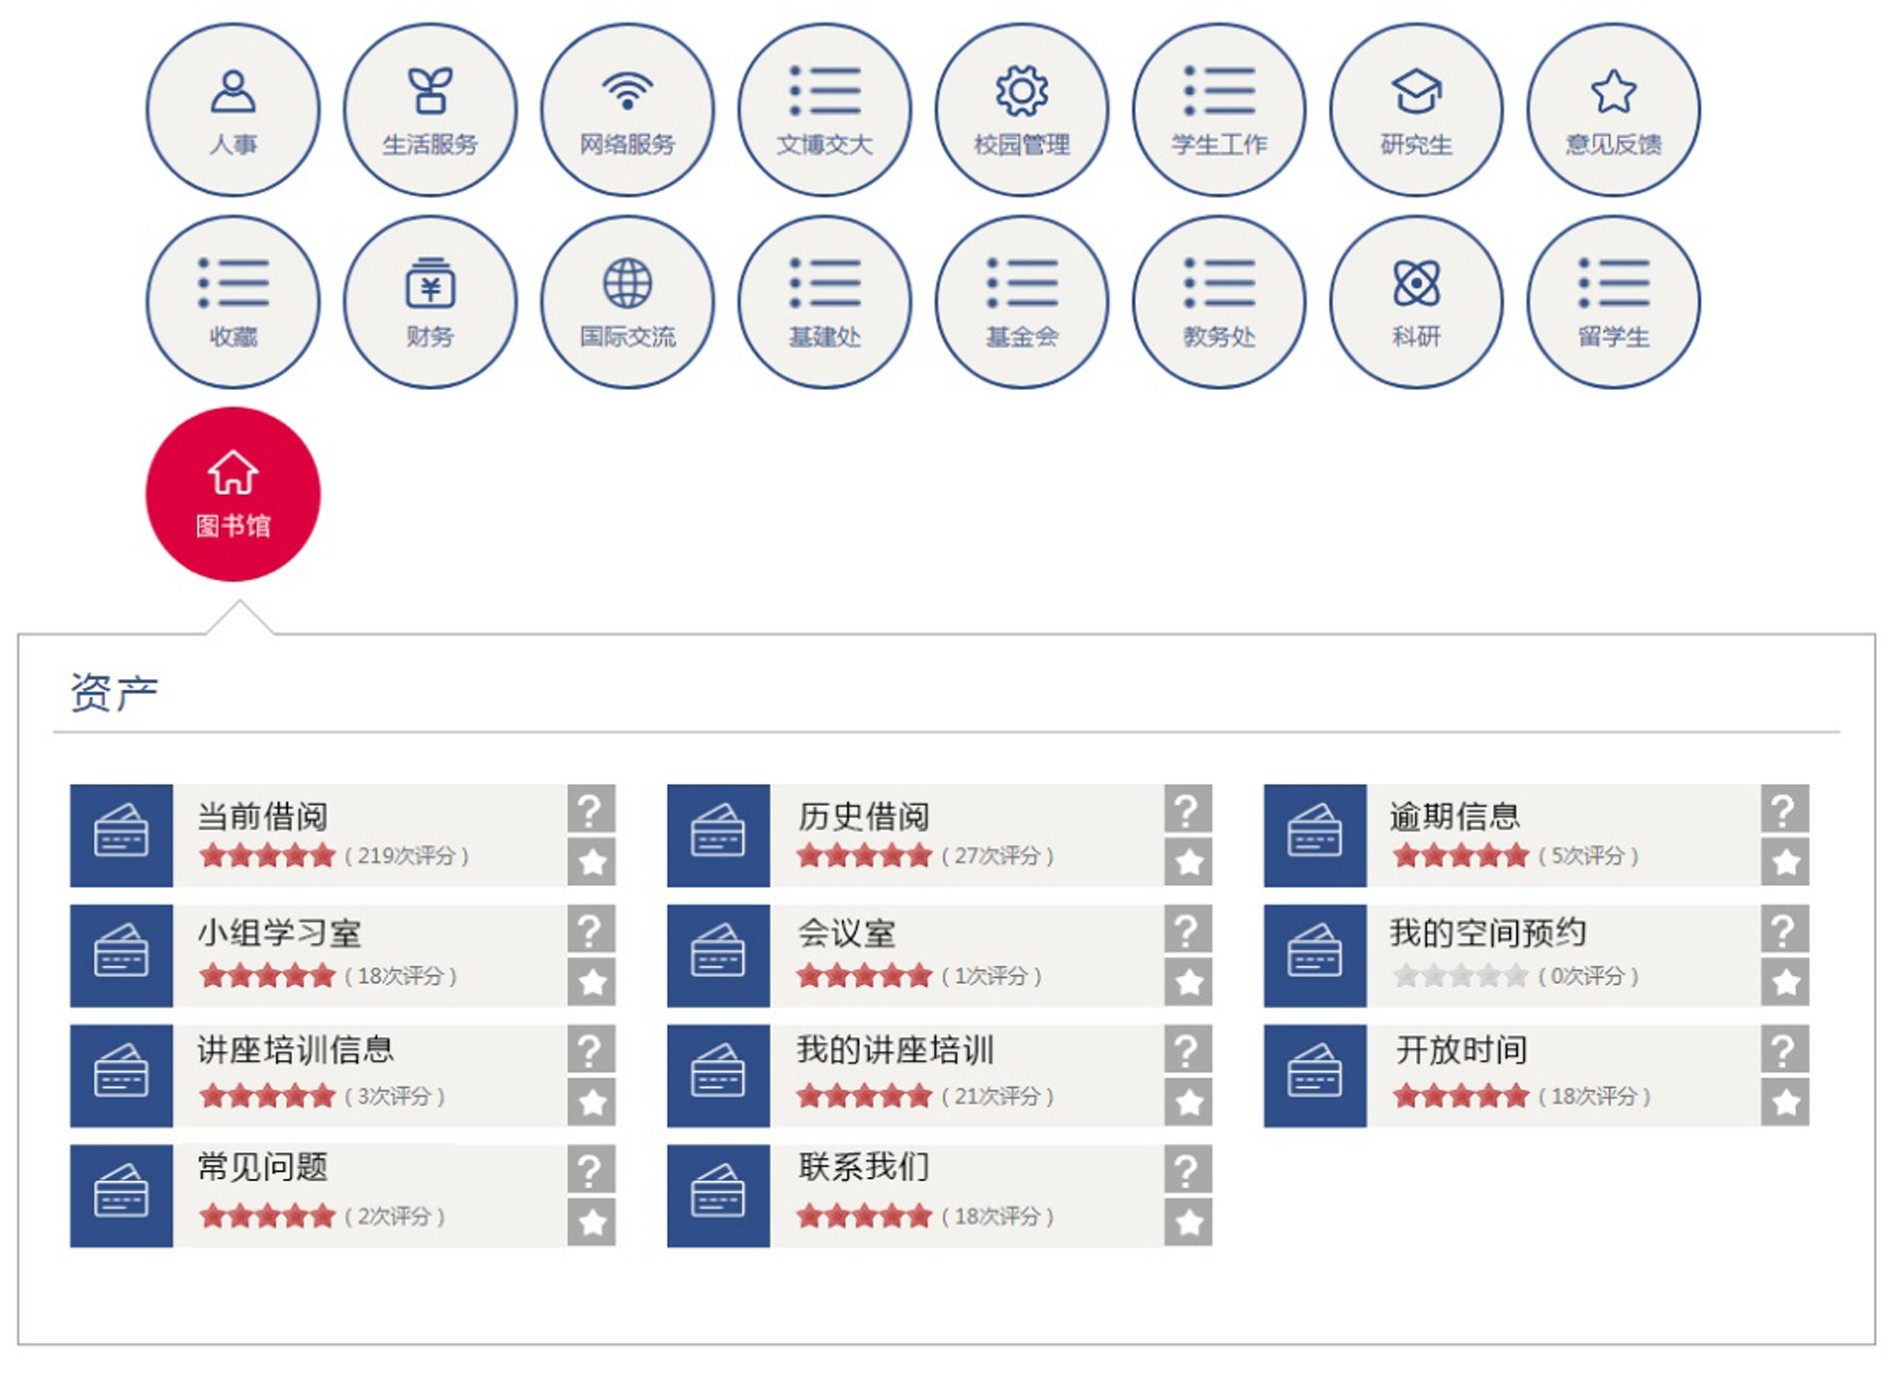
\includegraphics[height=0.4\textheight]{pic3.jpg}
	\caption{系统组成}
	\label{pic:3}
\end{figure}

\chapter{主要功能模块}

\section{类}

\subsection{账户类}

账户类涉及到一个$ Account $作为父类,$ User $、$ Guest $和$ Admin $三个子类。

\subsection{书本类}

书本类涉及到一个$ Book $作为父类,$Calendars$、$Children's Books$、$Computers$、$Engineering$和$Dieting$。

\section{登录\&注册}

本软件的登录和注册功能集成在一个界面,当用户输入完账号密码以后,若他想要注册,那么点击注册即可。

\subsection{类}

登录界面使用了login类。

\subsection{界面}
其界面如图\ref{pic:4}所示。

\begin{figure}[!htbp]
	\centering
	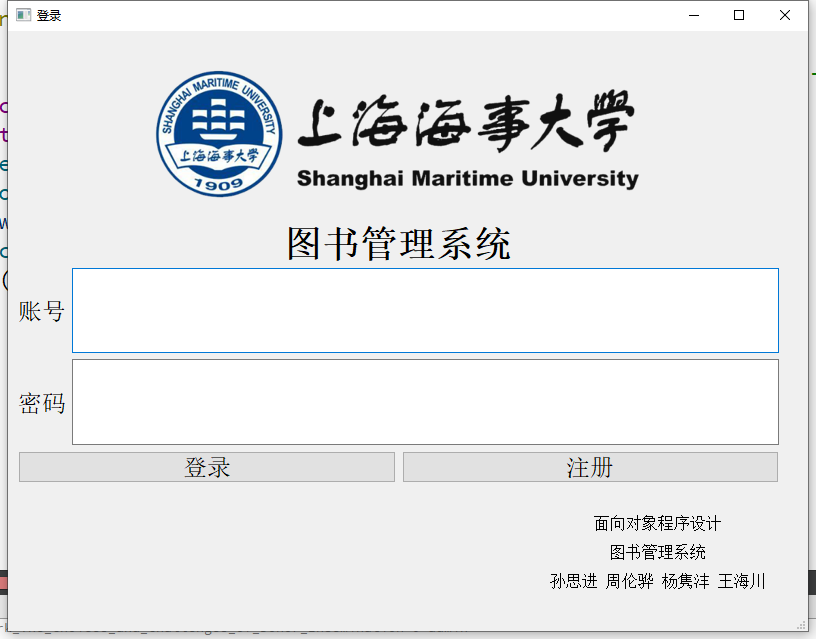
\includegraphics[height=0.3\textheight]{pic4.png}
	\caption{登录和注册界面}
	\label{pic:4}
\end{figure}

\subsection{实现}

成员函数主要涉及到登录、注册、查询数据、写入数据的功能。

\begin{lstlisting}[language=C++]
#include "login.h"
#include "ui_login.h"
#include "iostream"
#include "bookui.h"

Login::Login(QWidget *parent)
: QMainWindow(parent)
, ui(new Ui::Login)
{
	ui->setupUi(this);
}

Login::~Login()
{
	delete ui;
}

void Login::on_login_clicked()
{
	QString acc = this->ui->account->toPlainText();
	QString pas = this->ui->passowrd->toPlainText();
	string a = acc.toStdString();
	string p = pas.toStdString();
	if (this->Acc->compare(a,p))
	{
		bookui *p = nullptr;
		p =  new bookui;
		p->setPath(this->Acc->getPath());
		p->setAccount(this->Acc);
		p->setLogin(a,this->Acc->getAuthByAcc(a));
		p->ShowName(a);
		p->show();
	}
	else if(!this->Acc->compareAcc(a))
	{
		error *err = new error;
		err->show();
		err->ShowText("账号不存在");
	}
	else
	{
		error *err = new error;
		err->show();
		err->ShowText("密码错误");
	}
}

void Login::on_regist_clicked()
{
	QString acc = this->ui->account->toPlainText();
	QString pas = this->ui->passowrd->toPlainText();
	string a = acc.toStdString();
	string p = pas.toStdString();
	if(!this->Acc->compareAcc(a))
	{
		this->Acc->addUser(a,p,0);
		error *err = new error;
		err->show();
		err->ShowText("注册成功");
		qDebug("success");
	}
	else if(a.length()<=5 or p.length()<=5)
	{
		error *err = new error;
		err->show();
		err->ShowText("账号或密码太短,请重新输入");
		this->ui->account->clear();
		this->ui->passowrd->clear();
		qDebug("unsuccess");
	}
	else
	{
		error *err = new error;
		this->ui->account->clear();
		this->ui->passowrd->clear();
		err->show();
		err->ShowText("注册失败,账号重复");
		qDebug("unsuccess");
	}
	
}

void Login::AddAccount(Account *a)
{
	this->Acc = a;
}
\end{lstlisting}

本软件通过登录和注册两个按钮,即QT中的槽和信号的模块实现进入下一个窗口的功能。

登录需要根橱读者或管理员提供的登录账号和密码进行.系统会自动)进行后台数据库的验证,并根据错误信息返回登录,在登录模块进行权限验证,用于区分读者身份和管理员身份。登录模块效果如圈3所示。
读者模块主要包含关于读者仅限的操作。用户登录后会直接跳转到个人信息页面也可以跳转到其他用户的操作页面主要包括个人信息、图书查阅和密码修改三个小模块。个人信息模块主要显示个人基础信息以及当前书籍借阅和历史书籍借阅情况。

图书查询模块会根据读者输入的信息按类别进行检索查询,将检索结果进行分页显示,便于用户查阅。

\subsection{提示}

当用户输入了错误的账号或者密码,软件的提示如图\ref{pic:5}所示。

\begin{figure}[!htbp]
	\centering
	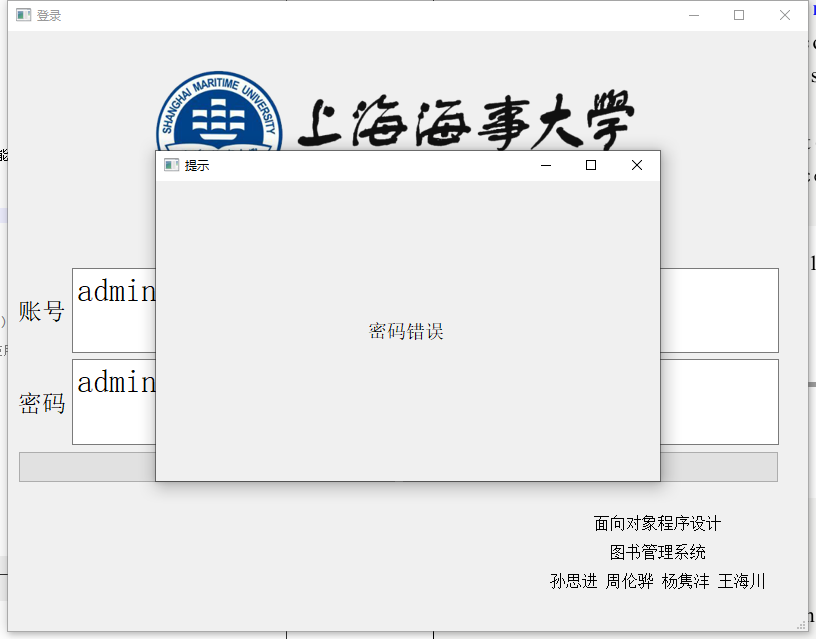
\includegraphics[height=0.2\textheight]{pic5.png}
	\caption{密码错误}
	\label{pic:5}
\end{figure}

当用户想要注册账号时,输入的账号已经存在,那么会提示账号已存在,如图\ref{pic:6}所示。

\begin{figure}[!htbp]
	\centering
	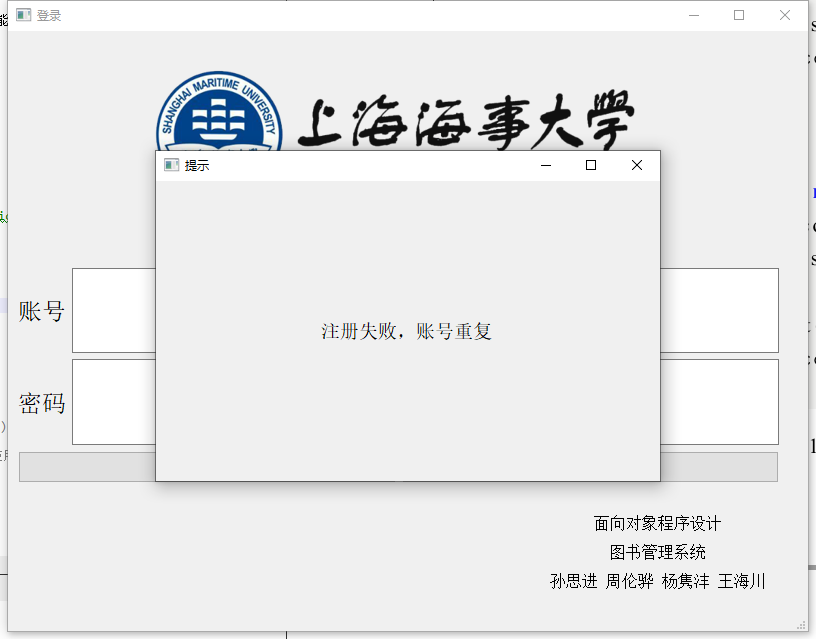
\includegraphics[height=0.2\textheight]{pic6.png}
	\caption{账号已存在}
	\label{pic:6}
\end{figure}

当用户注册账号成功时,保留原始输入的账号、密码和界面,软件读取输入的字符串,存储到csv文件中,如图\ref{pic:7}所示,提示账号注册成功。

\begin{figure}[!htbp]
	\centering
	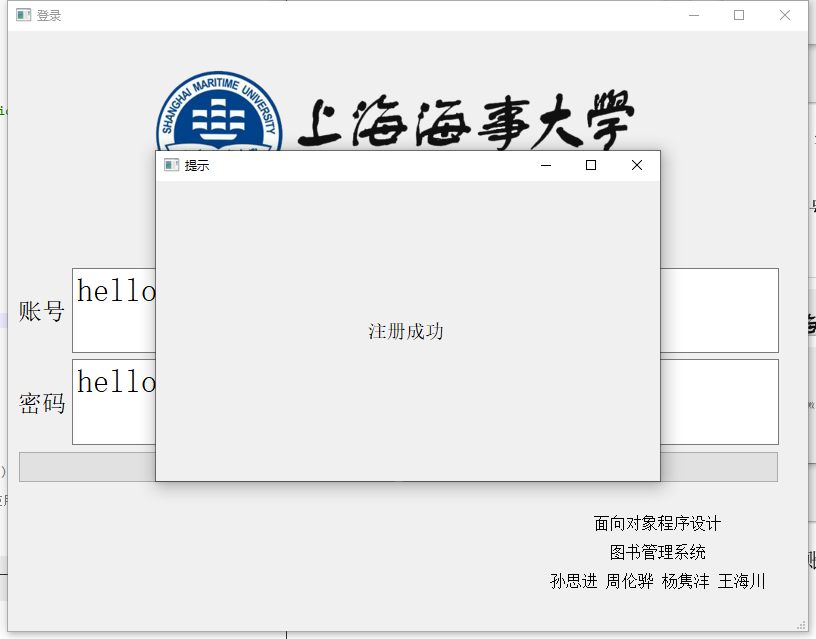
\includegraphics[height=0.2\textheight]{pic7.png}
	\caption{账号注册成功}
	\label{pic:7}
\end{figure}

当用户输入的账号和密码与csv文件中储存的数据一致时,弹出登陆成功的提示,跳转到主界面,如下文图\ref{pic:8}所示。

\section{主界面}

本软件的主界面设计了四个主要的功能:借书、查书、还书和管理员功能。

同时,软件在主界面显示了6本新书速递,展示了入库时间最晚的6本书。

\subsection{类}

主界面使用了Bookui类。

\subsection{界面}

主界面如图\ref{pic:8}所示,对于不同的登录用户,如图\ref{pic:9},会显示不同的管理员权限。

\begin{figure}[!htbp]
	\centering
	\begin{minipage}[!htbp]{0.45\linewidth}
		\centering
		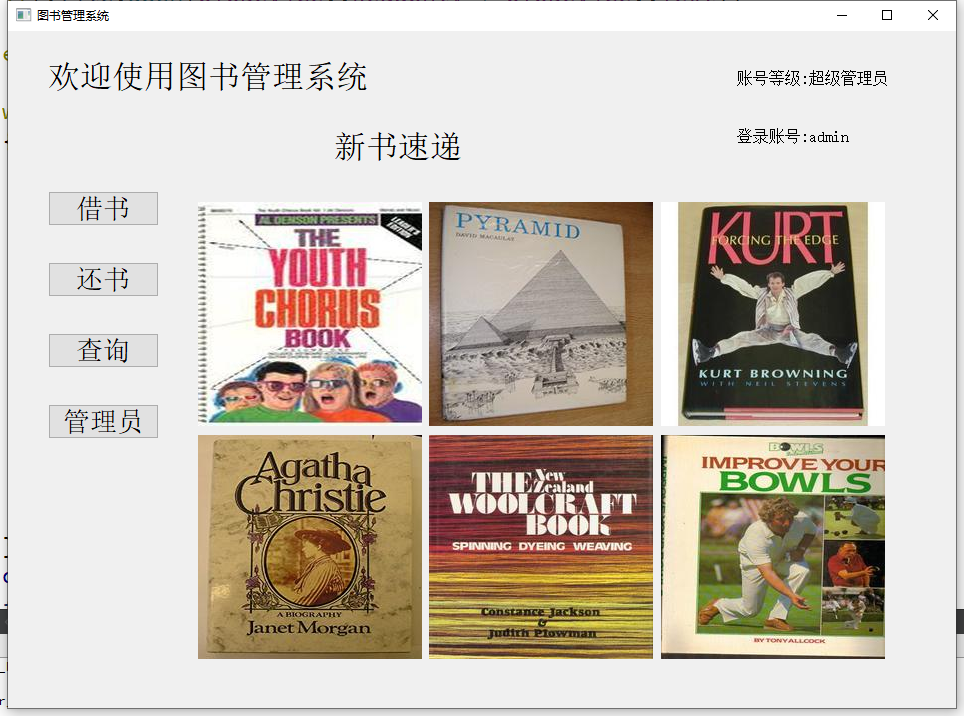
\includegraphics[height=0.2\textheight]{pic8.png}
		\caption{主界面-管理员}
		\label{pic:8}
	\end{minipage}%
	\begin{minipage}[!htbp]{0.45\linewidth}
		\centering
		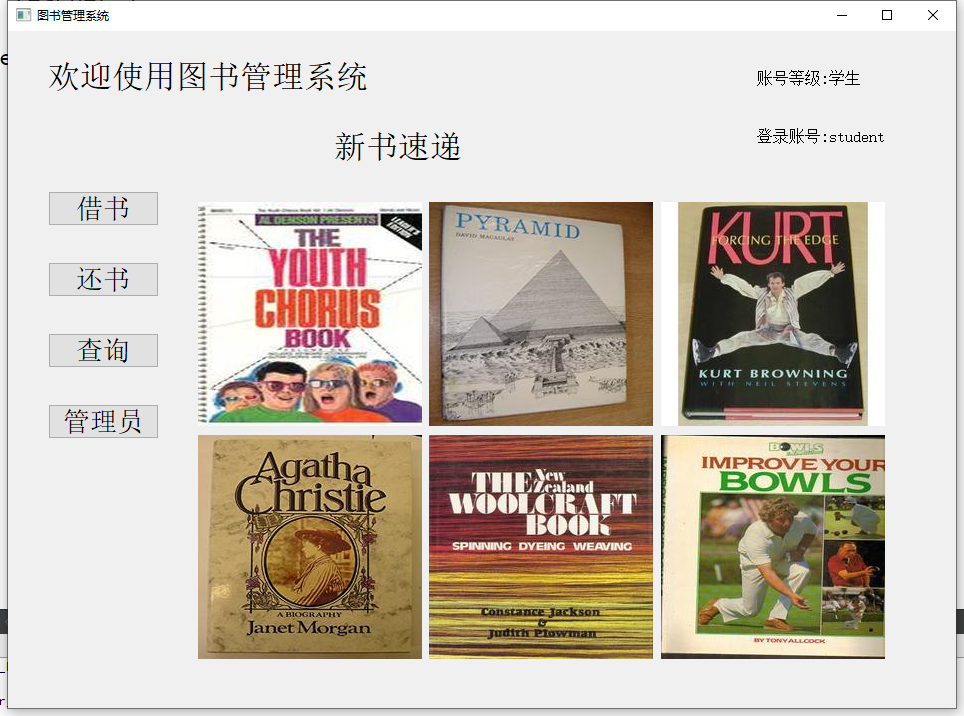
\includegraphics[height=0.2\textheight]{pic9.png}
		\caption{主界面-学生}
		\label{pic:9}
	\end{minipage}%
\end{figure}

\subsection{实现}

通过四个按钮,跳转到四个不同的功能界面。

由于图书涉及到多个不同的种类,我们将其分为$Calendars$、$Children's Books$、$Computers$、$Engineering$和$Dieting$。

\begin{lstlisting}[language=C++]
#include "bookui.h"
#include "ui_bookui.h"

bookui::bookui(QWidget *parent) :
QWidget(parent),
ui(new Ui::bookui)
{
	ui->setupUi(this);
}

bookui::~bookui()
{
	delete ui;
}

void bookui::setAccount(Account *a)
{
	this->Acc = a;
}

string bookui::getLoginAcc()
{
	return this->loginAcc;
}

void bookui::setLogin(string a,int b)
{
	this->loginAcc= a;
	this->loginAuth = b;
}

int bookui::getLoginAuth()
{
	return this->loginAuth;
}

void bookui::ShowName(string s)
{
	this->ui->AccountLabel->setText(QString::fromStdString("登录账号:" + s));
	string a;
	this->loginAuth = this->getLoginAuth();
	a = this->Acc->getAuthString(this->Acc->getAuthByAcc(s));
	this->ui->AuthLabel->setText(QString::fromStdString("账号等级:" + a));
	qDebug("是否运行");
	Book *d = new Book;
	d->add();
	d->setPath(this->Acc->getPath());
	this->setBook(d);
}

void bookui::setBook(Book *bo)
{
	this->book = bo;
}

void bookui::on_BorrowButton_clicked()
{
	if (this->getLoginAuth() >= 2)
	{
		borrow *c = new borrow;
		c->setBook(this->book);
		c->setLoginAccount(this->loginAcc);
		c->show();
	}
	else
	{
		error *e = new error;
		e->ShowText("非管理员权限只能使用查询和还书功能。");
		e->show();
	}
}

void bookui::on_LendButton_clicked()
{
	if (this->getLoginAuth() >= 2)
	{
		lend *l = new lend;
		l->setBook(this->book);
		l->show();
	}
	else
	{
		error *e = new error;
		e->ShowText("访客权限只能使用查询功能。");
		e->show();
	}
}

void bookui::on_AdminButton_clicked()
{
	if (this->getLoginAuth() >= 3)
	{
		auto *a = new admin;
		a->setAuthr(getLoginAuth());
		a->setAcc(this->Acc);
		a->show();
	}
	else
	{
		error *e = new error;
		e->ShowText("非超级管理员权限无法使用管理员功能。");
		e->show();
	}
}

void bookui::on_SearchButton_clicked()
{
	
	auto *s = new findd;
	s->setBook(this->book);
	s->show();
}

void bookui::setPath(string s)
{
	this->path = s;
}

string bookui::getPath()
{
	return this->path;
}
#include "lend.h"
#include "ui_lend.h"

lend::lend(QWidget *parent) :
QWidget(parent),
ui(new Ui::lend)
{
	ui->setupUi(this);
}

lend::~lend()
{
	delete ui;
}

void lend::setBook(Book *b)
{
	this->book = b;
}

void lend::on_SerachButton_clicked()
{
	qDebug("%d",1);
	QString SearchText = this->ui->SearchText->toPlainText();
	string s = SearchText.toStdString();
	qDebug("%d",2);
	int z = -1;
	for(int i = 0;i<this->book->getL();i++)
	{
		if(this->book->getName(i) == s || this->book->getISBN(i) == s)
		{
			z = i;
			break;
		}
	}
	
	if (z == -1)
	{
		error *p = new error;
		p->show();
		p->ShowText("找不到此信息,请重新输入");
		this->ui->SearchText->clear();
	}
	else
	{
		this->ui->BookLabel->setPixmap(QString::fromStdString(":/img/img/book/" + this->book->getISBN(z) +".jpg"));
		if (this->book->getStatus(z))
		{
			this->book->setStatus(z,0);
			this->book->writeBook();
			error *p = new error;
			p->show();
			p->ShowText("还书成功");
		}
		else
		{
			error *p = new error;
			p->show();
			p->ShowText("书本未处于出借状态,请重新确认");
		}
	}
}
\end{lstlisting}

\section{借书}

借书界面主要实现的是借书和查询书的功能,当用户权限不是管理员时,无法使用该功能。

\subsection{类}

借书使用了borrow类。

\subsection{界面}

界面主要涉及到查询和借阅两个按钮,图书查询模块会根据读者输入的信息按类别进行检索查询,将检索结果进行分页显示,便于用户查阅。当用户按下查询时,界面的信息将会更新,如图\ref{pic:10}所示。

\begin{figure}[!htbp]
	\centering
	\begin{minipage}[!htbp]{0.45\linewidth}
		\centering
		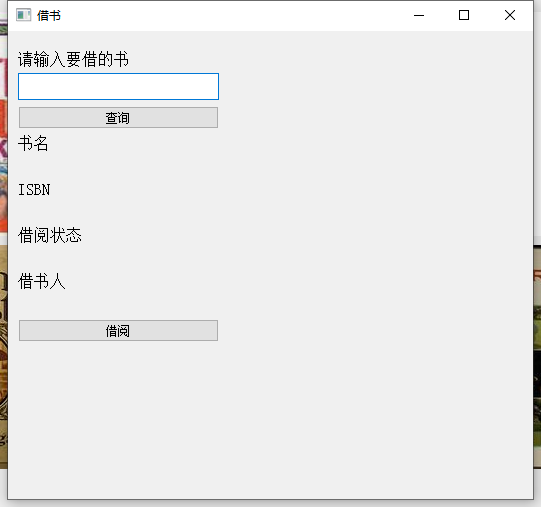
\includegraphics[height=0.2\textheight]{pic10.png}
		\caption{借书界面}
		\label{pic:10}
	\end{minipage}%
	\begin{minipage}[!htbp]{0.45\linewidth}
		\centering
		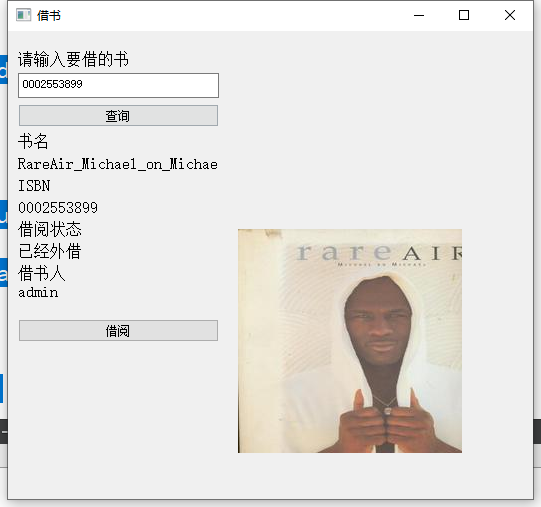
\includegraphics[height=0.2\textheight]{pic12.png}
		\caption{主界面-学生}
		\label{pic:12}
	\end{minipage}%
\end{figure}

当按下查询以后,会显示该本书的信息和书本封面,如图\ref{pic:12}所示。

\subsection{实现}

读者模块主要包含关于读者仅限的操作。用户登录后会直接跳转到个人信息页面也可以跳转到其他用户的操作页面主要包括个人信息、图书查阅和密码修改三个小模块。个人信息模块主要显示个人基础信息以及当前书籍借阅和历史书籍借阅情况。

该功能的实现主要依靠数据库的查询和修改,其成员函数如下:

\begin{lstlisting}[language=C++]
#include "bookui.h"
#include "ui_bookui.h"

bookui::bookui(QWidget *parent) :
QWidget(parent),
ui(new Ui::bookui)
{
	ui->setupUi(this);
}

bookui::~bookui()
{
	delete ui;
}

void bookui::setAccount(Account *a)
{
	this->Acc = a;
}

string bookui::getLoginAcc()
{
	return this->loginAcc;
}

void bookui::setLogin(string a,int b)
{
	this->loginAcc= a;
	this->loginAuth = b;
}

int bookui::getLoginAuth()
{
	return this->loginAuth;
}

void bookui::ShowName(string s)
{
	this->ui->AccountLabel->setText(QString::fromStdString("登录账号:" + s));
	string a;
	this->loginAuth = this->getLoginAuth();
	a = this->Acc->getAuthString(this->Acc->getAuthByAcc(s));
	this->ui->AuthLabel->setText(QString::fromStdString("账号等级:" + a));
	qDebug("是否运行");
	Book *d = new Book;
	d->add();
	d->setPath(this->Acc->getPath());
	this->setBook(d);
}

void bookui::setBook(Book *bo)
{
	this->book = bo;
}

void bookui::on_BorrowButton_clicked()
{
	if (this->getLoginAuth() >= 2)
	{
		borrow *c = new borrow;
		c->setBook(this->book);
		c->setLoginAccount(this->loginAcc);
		c->show();
	}
	else
	{
		error *e = new error;
		e->ShowText("非管理员权限只能使用查询和还书功能。");
		e->show();
	}
}

void bookui::on_LendButton_clicked()
{
	if (this->getLoginAuth() >= 2)
	{
		lend *l = new lend;
		l->setBook(this->book);
		l->show();
	}
	else
	{
		error *e = new error;
		e->ShowText("访客权限只能使用查询功能。");
		e->show();
	}
}

void bookui::on_AdminButton_clicked()
{
	if (this->getLoginAuth() >= 3)
	{
		auto *a = new admin;
		a->setAuthr(getLoginAuth());
		a->setAcc(this->Acc);
		a->show();
	}
	else
	{
		error *e = new error;
		e->ShowText("非超级管理员权限无法使用管理员功能。");
		e->show();
	}
}

void bookui::on_SearchButton_clicked()
{
	
	auto *s = new findd;
	s->setBook(this->book);
	s->show();
}

void bookui::setPath(string s)
{
	this->path = s;
}

string bookui::getPath()
{
	return this->path;
}
\end{lstlisting}

\subsection{提示}

若用户的权限不够,将无法打开结束界面,其提示如图所示。

\begin{figure}[!htbp]
	\centering
	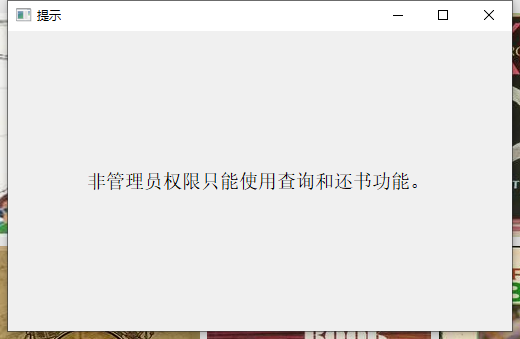
\includegraphics[height=0.2\textheight]{pic11.png}
	\caption{账号权限不够}
	\label{pic:11}
\end{figure}

\section{还书}

该界面主要为了做到还书的功能,通过查询数据库,先判断其是否属于借出状态,在进行还书,写入数据。

\subsection{类}

还书界面使用了Lend类。

\subsection{界面}

还书的界面如图\ref{pic:13}所示。

\begin{figure}[!htbp]
	\centering
	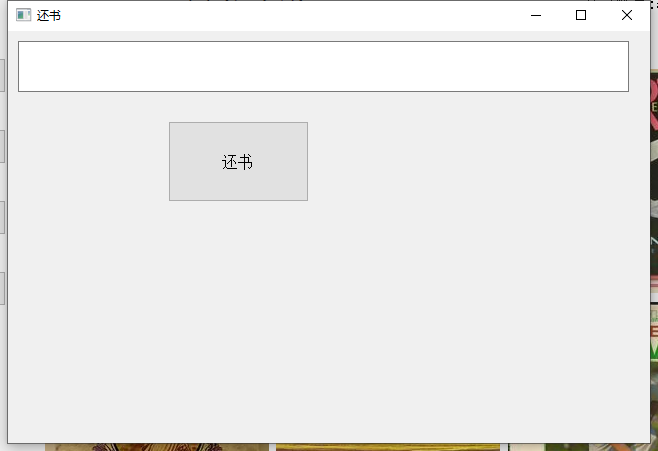
\includegraphics[height=0.2\textheight]{pic13.png}
	\caption{还书界面}
	\label{pic:13}
\end{figure}

\subsection{实现}

先调取用户输入的账号,查询数据库进行匹配,成员函数如下所示。

\begin{lstlisting}[language=C++]
#include "lend.h"
#include "ui_lend.h"

lend::lend(QWidget *parent) :
QWidget(parent),
ui(new Ui::lend)
{
	ui->setupUi(this);
}

lend::~lend()
{
	delete ui;
}

void lend::setBook(Book *b)
{
	this->book = b;
}

void lend::on_SerachButton_clicked()
{
	qDebug("%d",1);
	QString SearchText = this->ui->SearchText->toPlainText();
	string s = SearchText.toStdString();
	qDebug("%d",2);
	int z = -1;
	for(int i = 0;i<this->book->getL();i++)
	{
		if(this->book->getName(i) == s || this->book->getISBN(i) == s)
		{
			z = i;
			break;
		}
	}
	
	if (z == -1)
	{
		error *p = new error;
		p->show();
		p->ShowText("找不到此信息,请重新输入");
		this->ui->SearchText->clear();
	}
	else
	{
		this->ui->BookLabel->setPixmap(QString::fromStdString(":/img/img/book/" + this->book->getISBN(z) +".jpg"));
		if (this->book->getStatus(z))
		{
			this->book->setStatus(z,0);
			this->book->writeBook();
			error *p = new error;
			p->show();
			p->ShowText("还书成功");
		}
		else
		{
			error *p = new error;
			p->show();
			p->ShowText("书本未处于出借状态,请重新确认");
		}
	}
}
\end{lstlisting}

\subsection{提示}

还书的界面会出现三个提示,还书成功(图\ref{pic:14})、书本未处于借阅状态(图\ref{pic:15})和书本不存在(图\ref{pic:16})。

\begin{figure}[!htbp]
	\centering
	\begin{minipage}[!htbp]{0.33\linewidth}
		\centering
		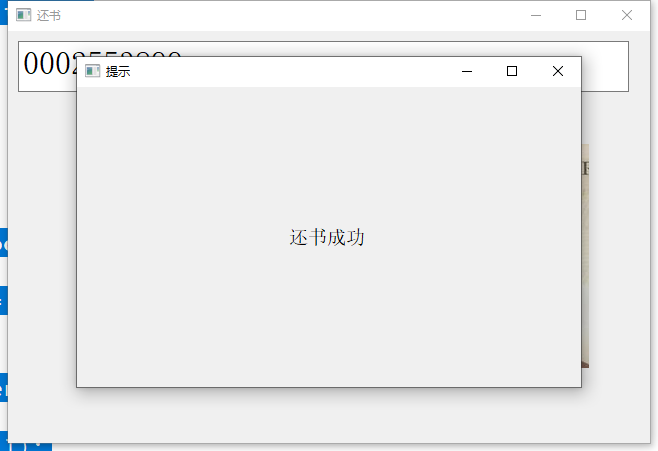
\includegraphics[height=0.13\textheight]{pic14.png}
		\caption{还书成功}
		\label{pic:14}
	\end{minipage}%
	\begin{minipage}[!htbp]{0.33\linewidth}
		\centering
		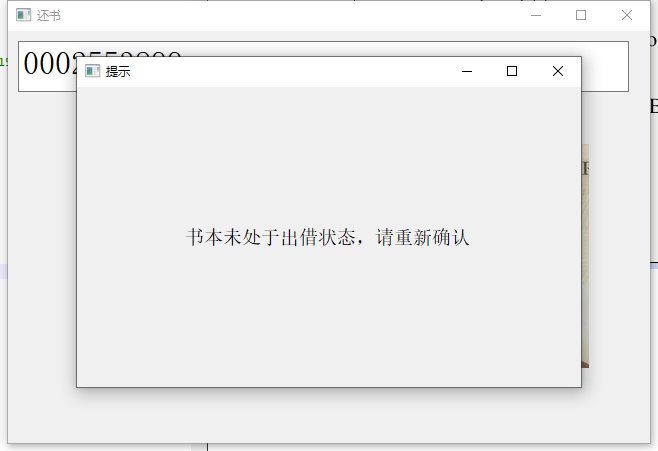
\includegraphics[height=0.13\textheight]{pic15.png}
		\caption{书本未借阅}
		\label{pic:15}
	\end{minipage}%
	\begin{minipage}[!htbp]{0.33\linewidth}
		\centering
		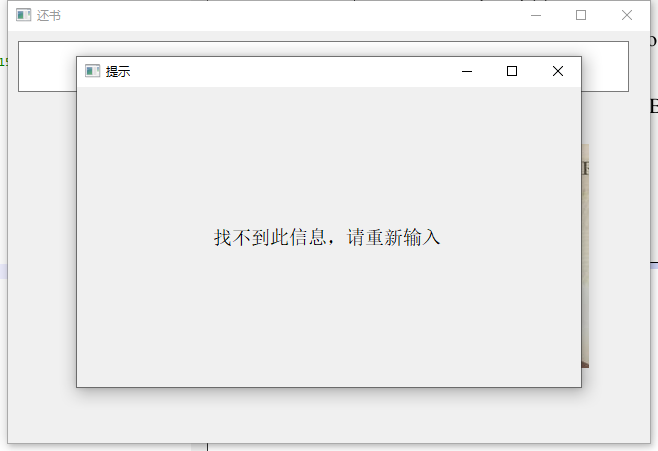
\includegraphics[height=0.13\textheight]{pic16.png}
		\caption{书本不存在}
		\label{pic:16}
	\end{minipage}%
\end{figure}

\section{查询}

查询功能是借书的继承功能,其功能大致与借书类似,由于查询功能可供访客使用,消去了显示借阅者的功能,如图\ref{pic:17}所示。

\subsection{类}

查询使用了search类。

\subsection{界面}

图书查询模块会根据读者输入的信息按类别进行检索查询, 将检索结果进行分页显示, 便于用户查阅。

\begin{figure}[!htbp]
	\centering
	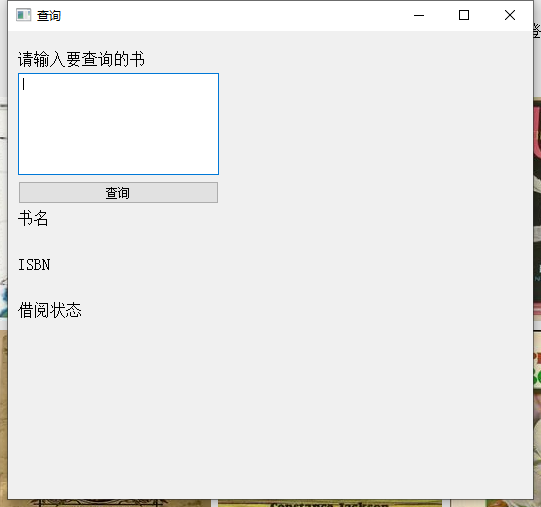
\includegraphics[height=0.2\textheight]{pic17.png}
	\caption{查询界面}
	\label{pic:17}
\end{figure}

\section{管理员}

超级管理员是管理员中最大的权限,他可以控制除了他以外的用户进行升降级权限。

\subsection{类}

管理员使用了Admin类。

\subsection{界面}

管理员界面主要有查询账号(图\ref{pic:18})、修改密码(图\ref{pic:19})、修改权限的功能。先查询账号,再显示其信息,如图\ref{pic:18}所示。

\begin{figure}[!htbp]
	\centering
	\begin{minipage}[!htbp]{0.33\linewidth}
		\centering
		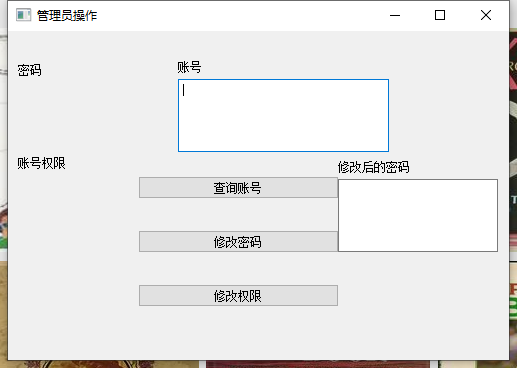
\includegraphics[height=0.13\textheight]{pic18.png}
		\caption{管理员界面}
		\label{pic:18}
	\end{minipage}%
	\begin{minipage}[!htbp]{0.33\linewidth}
		\centering
		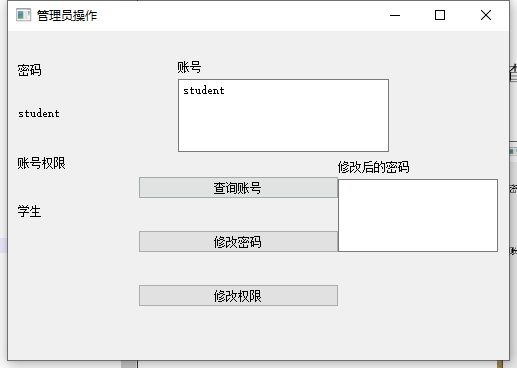
\includegraphics[height=0.13\textheight]{pic19.png}
		\caption{查询账号和权限}
		\label{pic:19}
	\end{minipage}%
	\begin{minipage}[!htbp]{0.33\linewidth}
		\centering
		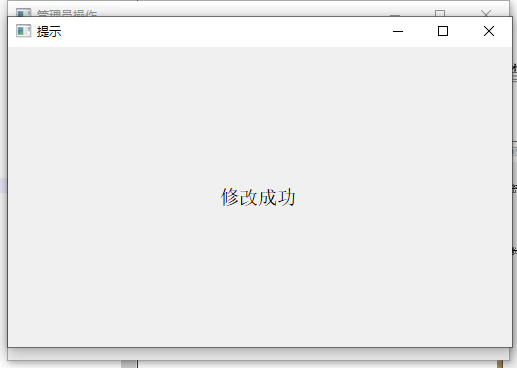
\includegraphics[height=0.13\textheight]{pic20.png}
		\caption{修改密码}
		\label{pic:20}
	\end{minipage}%
\end{figure}

\subsection{实现}

对于上述三个功能,实现了查询账号、修改密码、修改权限的功能。

\begin{lstlisting}[language=C++]
#include "admin.h"
#include "ui_admin.h"

admin::admin(QWidget *parent) :
QWidget(parent),
ui(new Ui::Admin)
{
	ui->setupUi(this);
}

admin::~admin()
{
	delete ui;
}

void admin::on_AccountButton_clicked()
{
	QString acc = this->ui->AccountText->toPlainText();
	string ac = acc.toStdString();
	int z = -1;
	qDebug("%d",this->Acc->getL());
	for(int i =0; i< this->Acc->getL();i++)
	{
		qDebug(qUtf8Printable(QString::fromStdString(this->Acc->getAcc(i))));
		if (ac == this->Acc->getAcc(i))
		{
			z = i;
			break;
		}
	}
	qDebug("%d",z);
	if(z+1)
	{
		this->ui->PasswordLabel->setText(QString::fromStdString(this->Acc->getPas(z)));
		this->ui->AuthLabel->setText(QString::fromStdString(this->Acc->getAuthString(this->Acc->getAuth(z))));;
	}
	else
	{
		error *e = new error;
		e->ShowText("未找到此账号");
		e->show();
	}
}

void admin::setAcc(Account *a)
{
	this->Acc = a;
}

void admin::on_PasswordButton_clicked()
{
	QString s = this->ui->AccountText->toPlainText();
	string ss = s.toStdString();
	string pas = this->ui->PasswordSet->toPlainText().toStdString();
	int z = -1;
	qDebug("%d",this->Acc->getL());
	for(int i =0; i< this->Acc->getL();i++)
	if (ss == this->Acc->getAcc(i))
	{
		z = i;
		break;
	}
	
	qDebug("%d",z);
	if (pas.length()<5)
	{
		error *e = new error;
		e->ShowText("密码长度过短,请重新输入");
		e->show();
		this->ui->PasswordLabel->clear();
		this->ui->PasswordSet->clear();
	}
	else if(z+1)
	{
		error *e = new error;
		e->ShowText("修改成功");
		e->show();
		this->Acc->setPas(z,pas);
		this->ui->PasswordLabel->setText(QString::fromStdString(pas));
		this->Acc->save();
	}
	else
	{
		error *e = new error;
		e->ShowText("未找到此账号");
		e->show();
	}
}

void admin::on_AuthButton_clicked()
{
	if(this->getAuthr() >=3)
	{
		auth *a = new auth;
		a->setAcc(this->Acc);
		a->show();
	}
	else
	{
		error *e = new error;
		e->ShowText("普通管理员无法修改权限");
		e->show();
	}
}

void admin::setAuthr(int a)
{
	this->authr = a;
}

int admin::getAuthr()
{
	return this->authr;
}
\end{lstlisting}

\section{升\&降级}

通过点击修改权限的按钮,进入升降级功能。

\subsection{类}

升降级使用了auth类。

\subsection{界面}

其界面如图\ref{pic:21}所示。

\begin{figure}[!htbp]
	\centering
	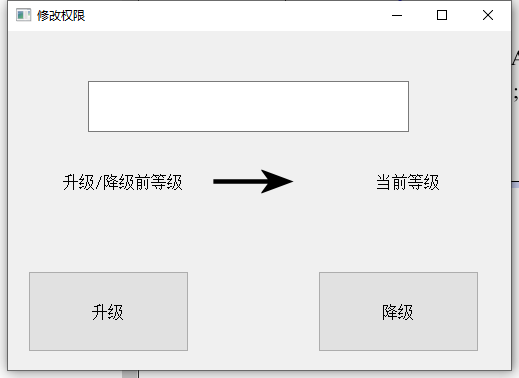
\includegraphics[height=0.2\textheight]{pic21.png}
	\caption{升降级}
	\label{pic:21}
\end{figure}

\subsection{实现}

对于一个用户,无法升级到超级管理员,也无法降级到访客以下。

\begin{lstlisting}[language=C++]
#include "auth.h"
#include "ui_auth.h"

auth::auth(QWidget *parent) :
QWidget(parent),
ui(new Ui::auth)
{
	ui->setupUi(this);
}

auth::~auth()
{
	delete ui;
}

void auth::setAcc(Account *a)
{
	this->Acc = a;
}
void auth::on_up_clicked()
{
	QString s = this->ui->textEdit->toPlainText();
	string ss = s.toStdString();
	int z = -1;
	qDebug("%d",this->Acc->getL());
	for(int i =0; i< this->Acc->getL();i++)
	if (ss == this->Acc->getAcc(i))
	{
		z = i;
		break;
	}
	if(z + 1)
	{
		if(this->Acc->getAuth(z) < 2)
		{
			this->Acc->setAuth(z,this->Acc->getAuth(z) + 1);
			this->Acc->save();
			error *e = new error;
			e->ShowText("权限升级成功");
			e->show();
			this->ui->now->setText(QString::fromStdString(this->Acc->getAuthString(this->Acc->getAuth(z))));
			this->ui->present->setText(QString::fromStdString(this->Acc->getAuthString(this->Acc->getAuth(z) - 1)));
		}
		else
		{
			error *e = new error;
			e->ShowText("该账户已经是普通管理员权限,无法升级");
			e->show();
			this->ui->now->setText(QString::fromStdString(this->Acc->getAuthString(this->Acc->getAuth(z))));
			this->ui->present->clear();
		}
	}
}

void auth::on_down_clicked()
{
	QString s = this->ui->textEdit->toPlainText();
	string ss = s.toStdString();
	int z = -1;
	qDebug("%d",this->Acc->getL());
	for(int i =0; i< this->Acc->getL();i++)
	if (ss == this->Acc->getAcc(i))
	{
		z = i;
		break;
	}
	if(z + 1)
	{
		if(this->Acc->getAuth(z) < 2 && this->Acc->getAuth(z) > 0)
		{
			qDebug("%d等级",this->Acc->getAuth(z));
			this->Acc->setAuth(z,this->Acc->getAuth(z)-1);
			this->Acc->save();
			error *e = new error;
			e->ShowText("权限降级成功");
			e->show();
			this->ui->now->setText(QString::fromStdString(this->Acc->getAuthString(this->Acc->getAuth(z))));
			this->ui->present->setText(QString::fromStdString(this->Acc->getAuthString(this->Acc->getAuth(z + 1))));
		}
		
		else if(this->Acc->getAuth(z) == 3)
		{
			error *e = new error;
			e->ShowText("超级管理员无法降级");
			e->show();
			this->ui->now->setText(QString::fromStdString(this->Acc->getAuthString(this->Acc->getAuth(z))));
			this->ui->present->clear();
		}
		
		else
		{
			error *e = new error;
			e->ShowText("该账户已经是访客权限,无法降级");
			e->show();
			this->ui->now->setText(QString::fromStdString(this->Acc->getAuthString(this->Acc->getAuth(z))));
			this->ui->present->clear();
		}
	}
}

\end{lstlisting}

\chapter{数据结构说明}

\section{界面类}

\subsection{登录}

\begin{lstlisting}
#include <QMainWindow>
#include "account.h"
#include "error.h"
QT_BEGIN_NAMESPACE
namespace Ui { class Login; }
using namespace std;
QT_END_NAMESPACE

class Login : public QMainWindow
{
	Q_OBJECT
	
	public:
	Login(QWidget *parent = nullptr);
	~Login();
	void AddAccount(Account *a);
	
	public slots:
	void on_login_clicked();
	void on_regist_clicked();
	private:
	Ui::Login *ui;
	Account *Acc;
};
\end{lstlisting}

\subsection{账户}

\begin{lstlisting}
#include "fstream"
#include "QFile"
#include "string"
#include <QFileDialog>
#include <QMainWindow>
#include <QDebug>

#define MAXACCOUNT 100
using namespace std;

class Account
{
	private:
	string acc[MAXACCOUNT];
	string pas[MAXACCOUNT];
	int auth[MAXACCOUNT];//0访客 1学生 2老师 3普通管理员 4总管理员
	int l;
	string path;
	public:
	Account();
	string getAcc(int i);
	string getPas(int i);
	int getAuth(int i);
	void addUserLoad(string a,string p,int u);
	void addUser(string a,string p,int u);
	void save();
	int getL();
	bool compareAcc(string s);
	bool comparePas(string s);
	bool compare(string s1,string s2);
	void load();
	int getAuthByAcc(string a);
	void setPas(int i,string s);
	void setPath(string s);
	string getPath();
	void setAuth(int i,int j);
	string getAuthString(int i);
};
\end{lstlisting}

\subsection{书本}

\begin{lstlisting}
#include "string"
#include "QDebug"
#include "QFile"
#include "QString"
#include "error.h"
using namespace std;

class Book
{
	private:
	string ISBN[100];
	string name[100];
	bool status[100];
	string borrower[100];
	int no[100];
	int l;
	public:
	void addBook(string i,string n,bool s, string b,int no);
	void add();
	int getL();
	string getISBN(int i);
	string getName(int i);
	bool getStatus(int i);
	string getBorrower(int i);
	int getNo(int i);
	void writeBook();
	void setBorrower(int i,string s);
	void setStatus(int i,int s);
	string path;
	string getPath();
	void setPath(string s);
};
\end{lstlisting}

\chapter{总结}

在图书管理系统软件开发的过程中,从系统的规划到分析,再到系统设计、实施、运行和测评等一系列开发步骤,都严格按照软件开发波程进行,同时,在开发的过程中),对原有的初步方案不断修改经过反复调试,系统可实现登录、注册、图书管理、读者管理、借阅管理以及新书订购等功能、运行结果表明,该系统可满足小型图书馆的书籍管理和借阅工作。下一步的工作是进一步扩展属软件功能。扩大应用范围,并进一步提高软件的安全性等指标,使图书管理系统的功能更加完善。

%%%=== 参考文献 ========%%%
\cleardoublepage\phantomsection
\addcontentsline{toc}{chapter}{参考文献}
\begin{thebibliography}{99}

  \bibitem{r1} 王玉庆.基于Java的图书查询系统设计与实现[J].信息与电脑(理论版),2021,33(02):138-140.

  \bibitem{r2} 李萍,李芳.基于B/S结构的医院图书管理系统的设计与实现[J].泰山学院学报,2013,35(03):88-93.

  \bibitem{r3} 曹定舟,陈云忠,缪毅.医院图书借阅管理系统的设计与应用[J].中国医疗设备,2009,24(04):90-91.

  \bibitem{r4} 刘帅. 图书管理信息系统的设计与实现[D].吉林大学,2011.

  \bibitem{r5} 王思楠.图书馆流通过程中遇到的部分问题以及解决办法——以天津市少年儿童图书馆为例[J].内蒙古科技与经济,2020(12):122-123.
\end{thebibliography}

% !Mode:: "TeX:UTF-8"
%%%%%%%%%%%%%%%%%%%%%%%%%%%%-------致谢--------%%%%%%%%%%%%%%%%%%%%%%%%%%%%%%%%

\acknowledgement
\addcontentsline{toc}{chapter}{致谢}

通过本课设任课老师金世双老师的指导,我们小组完成了本项课程设计。

感谢你, 感谢他和她, 感谢大家.

为期近一学期的论文写作和软件设计即将画上一个圆满的句号,在论文写作的过程中,从论文的选题到确定思路,从资料的搜集、提纲的拟定到内容的写作与修改,继而诸多观点的梳理。

论文的点评中总是闪烁着智慧的火花,与他的每次交谈我都能从中获益。他渊博的学识,敏锐的学术洞察力,严谨的治学态度,一丝不苟的负责精神,以及对学生孜孜不倦的教诲都给予了我极其深刻的印象,让我受益匪浅。在此,谨向金老师表示我最衷心地感谢和最诚挚的敬意。

同时,也向从课程设计来所有教授过我和帮助过我的教授老师表示感谢,感谢您们对我的谆谆教诲、耐心指导和无私的帮助。

感谢我的同学和朋友们,感谢你们在我论文写作过程中给予我的鼓励、关心和无私的帮助。

最后,衷心地感谢我的家人,感谢你们一直以来给予我的.支持和鼓励。










 %%%致谢

%%%-------------- 附录. 不需要可以删除.-----------
\appendix

\end{document}



